%%%%%%%%%%%%%%%%%%%%%%%%%%%%%%%%%%%%%%%%%
% Beamer Presentation
% LaTeX Template
% Version 1.0 (10/11/12)
%
% This template has been downloaded from:
% http://www.LaTeXTemplates.com
%
% License:
% CC BY-NC-SA 3.0 (http://creativecommons.org/licenses/by-nc-sa/3.0/)
%
%%%%%%%%%%%%%%%%%%%%%%%%%%%%%%%%%%%%%%%%%

%----------------------------------------------------------------------------------------
%	PACKAGES AND THEMES
%----------------------------------------------------------------------------------------

\documentclass{beamer}

\mode<presentation> {

% The Beamer class comes with a number of default slide themes
% which change the colors and layouts of slides. Below this is a list
% of all the themes, uncomment each in turn to see what they look like.

%\usetheme{default}
%\usetheme{AnnArbor}
%\usetheme{Antibes}
%\usetheme{Bergen}
%\usetheme{Berkeley}
%\usetheme{Berlin}
%\usetheme{Boadilla}
%\usetheme{CambridgeUS}
%\usetheme{Copenhagen}
%\usetheme{Darmstadt}
%\usetheme{Dresden}
%\usetheme{Frankfurt}
\usetheme{Goettingen}
%\usetheme{Hannover}
%\usetheme{Ilmenau}
%\usetheme{JuanLesPins}
%\usetheme{Luebeck}
%\usetheme{Madrid}
%\usetheme{Malmoe}
%\usetheme{Marburg}
%\usetheme{Montpellier}
%\usetheme{PaloAlto}
%\usetheme{Pittsburgh}
%\usetheme{Rochester}
%\usetheme{Singapore}
%\usetheme{Szeged}
%\usetheme{Warsaw}

% As well as themes, the Beamer class has a number of color themes
% for any slide theme. Uncomment each of these in turn to see how it
% changes the colors of your current slide theme.

%\usecolortheme{albatross}
%\usecolortheme{beaver}
%\usecolortheme{beetle}
%\usecolortheme{crane}
%\usecolortheme{dolphin}
%\usecolortheme{dove}
%\usecolortheme{fly}
%\usecolortheme{lily}
%\usecolortheme{orchid}
%\usecolortheme{rose}
%\usecolortheme{seagull}
%\usecolortheme{seahorse}
%\usecolortheme{whale}
%\usecolortheme{wolverine}

%\setbeamertemplate{footline} % To remove the footer line in all slides uncomment this line
%\setbeamertemplate{footline}[page number] % To replace the footer line in all slides with a simple slide count uncomment this line

%\setbeamertemplate{navigation symbols}{} % To remove the navigation symbols from the bottom of all slides uncomment this line
}

\usepackage{graphicx} % Allows including images
\usepackage{booktabs} % Allows the use of \toprule, \midrule and \bottomrule in tables

%----------------------------------------------------------------------------------------
%	TITLE PAGE
%----------------------------------------------------------------------------------------

\title[3 Physics Experiments]{3 Simple Physics Experiments} % The short title appears at the bottom of every slide, the full title is only on the title page

\author{Preetha and Atul} % Your name
\institute[IISER M] % Your institution as it will appear on the bottom of every slide, may be shorthand to save space
{
Indian Institute of Science Education and Research Mohali \\ % Your institution for the title page
\medskip
% \textit{ms10024@iisermohali.ac.in} \\
% \textit{ms11003@iisermohali.ac.in} % Your email address
}
\date{\today} % Date, can be changed to a custom date

\begin{document}

\begin{frame}
\titlepage % Print the title page as the first slide
\end{frame}

\section{Outline}
\begin{frame}
\frametitle{Overview of the Talk} % Table of contents slide, comment this block out to remove it
\tableofcontents % Throughout your presentation, if you choose to use \section{} and \subsection{} commands, these will automatically be printed on this slide as an overview of your presentation
\end{frame}

\section{Introduction}
\begin{frame}
	\frametitle{School Physics}
		\begin{itemize}
			\item Optics
			\item Fluids
			\item Mechanics
			\item Electrodynamics*
			\item Thermodynamics*
			\item Modern Physics*
		\end{itemize}
\end{frame}

\section{The Wicked Shadow}
	\begin{frame}
		1. Optics
		\Huge{\centerline{The Wicked Shadow}}
		\tiny{\centerline{first demonstrated to us by Prof. Arvind}}
	\end{frame}

	\subsection{The Problem}
		\begin{frame}
		\frametitle{The Setup}
			There's a bright light source. There's a cardboard with a triangular hole. The cardboard blocks light from the light source to cast a shadow on a screen.
			\begin{figure}
			\includegraphics[width=0.8\linewidth]{images/WickedShadow}
			\end{figure}
		\end{frame}

	\subsection{The Demonstration}
		\begin{frame}
			\Large{\centerline{The Demonstration}}
		\end{frame}

	\subsection{The Explanation}
		\begin{frame}
		\frametitle{The Explanation}
			\Large{\centerline{Pinhole Camera}}
		\end{frame}

		\begin{frame}
		\frametitle{The Explanation}
			\begin{figure}				
			
\includegraphics[width=0.8\linewidth]{images/wickedShadow2}
			\end{figure}
		\end{frame}

		\begin{frame}
		\frametitle{The Explanation}
			\begin{figure}				
			
\includegraphics[width=0.8\linewidth]{images/wickedShadow3}
			\end{figure}
		\end{frame}

		\begin{frame}
		\frametitle{The Explanation}
			\begin{figure}				
			
\includegraphics[width=0.8\linewidth]{images/wickedShadow4}
			\end{figure}
		\end{frame}


\section{The Nut Spinner}
	\begin{frame}
		2. Mechanics
		\Huge{\centerline{The Nut Spinner}}		
		\tiny{\centerline{first demonstrated to us by Dr. Ravi Mehrotra}}
		\tiny{\centerline{conceived by Dr. Arvind Gupta}}
	\end{frame}

	\subsection{The Problem}
		\begin{frame}
		\frametitle{The Setup}
			Imagine a steel loop with a 1 foot diameter. There are some (say 4) nuts passing through the loop. You spin the nuts and rotate the ring as shown in the figure.
			\begin{figure}
			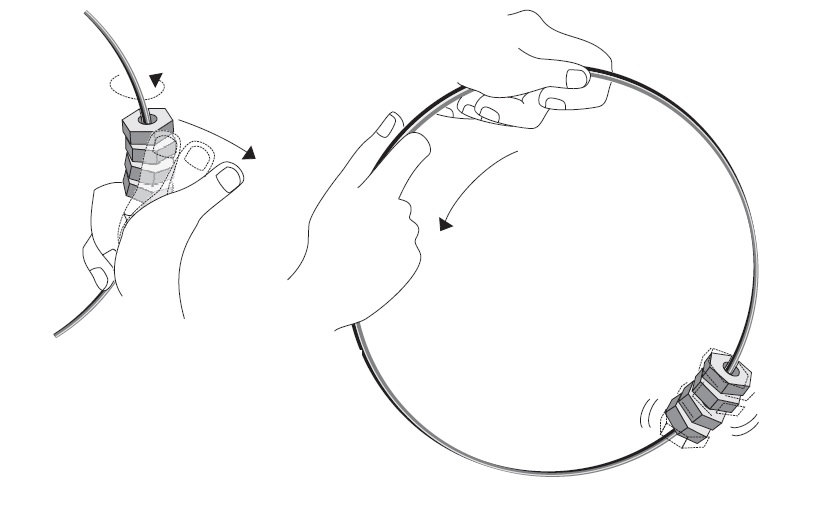
\includegraphics[width=0.8\linewidth]{images/nutspinner}
			\end{figure}
		\end{frame}

	\subsection{The Demonstration}
		\begin{frame}
			\Large{\centerline{The Demonstration}}
		\end{frame}

		\begin{frame}
		\frametitle{Simple Questions}
			\begin{enumerate}			
				\item What is the direction of torque being applied (by us)?
				\item What is the direction of the angular momentum of the nut?
				\item Can we neglect friction?
				\item How is the energy being transferred?
			\end{enumerate}
		\end{frame}

	\subsection{The Explanation}
		\begin{frame}
		\frametitle{The Explanation}
			Think about it.
		\end{frame}

\section{The Mystery Worker}
	\begin{frame}
		3. Fluids
		\Huge{\centerline{The Mystery Worker}}
		\tiny{\centerline{we were first asked by Dr. Mukun Thattai}}
	\end{frame}

	\subsection{The Problem}
		\begin{frame}
		\frametitle{The Setup}
			Consider a cylindrical jar containing water as shown in the figure. A rectangular membrane is placed in the cylinder along the diameter of its circular cross-section, such that the water is divided into two equal parts.
			\begin{figure}
			
\includegraphics[width=0.8\linewidth]{images/jarOfWater}
			\end{figure}
		\end{frame}

		\begin{frame}
		\frametitle{Simple Questions}
			\begin{enumerate}			
				\item What happens if salt is added to a partition?
				\item Is there any work done?
				\item If yes, who's doing the work?
			\end{enumerate}
		\end{frame}

	\subsection{The Demonstration}
		\begin{frame}
			\Large{\centerline{The Demonstration}}
		\end{frame}

	\subsection{The Explanation}
		\begin{frame}
		\frametitle{The Explanation}
			\begin{figure}
			
\includegraphics[width=0.8\linewidth]{images/jarOfWaterE}
			\end{figure}
		\end{frame}

		\begin{frame}
		\frametitle{The Explanation}
			Let there be $n_0$ moles of solvent and $n_1$ moles of solute in the solution.

			Free energy of the solution
			\begin{equation}
				A=U-TS
			\end{equation}
			Where the internal energy $U=U(T,P,n_0,n_1)$.
			Using taylor series we have

			\begin{equation}
				U(T,P,n_0,n_1)=U(T,P,n_0,0) + n_1 \frac {\partial U}{\partial n_1} + ...
			\end{equation}

			Assuming homogeneity

			\begin{equation}
				U(T,P,n_0,n_1) = n_0 u_0(T,P) + n_1 u_1(T,P)
			\end{equation}
			\begin{equation}
				V(T,P,n_0,n_1) = n_0 v_0 (T,P) + n_1 v_1 (T,P)
			\end{equation}

			where $u_0$ and $v_0$ are internal energy and volume per unit mol respectively.

		\end{frame}

		\begin{frame}
		\frametitle{The Explanation}
			Considering entropy

			\begin{equation}
				ds = \frac {dQ} {T} = \frac 1 T (dV + PdV)
				= n_0 \left[ \frac {du_0 + Pdv_0} {T}  + \frac {n_1} {n_0} \frac {du_1 + Pdv_1} {T} \right]
			\end{equation}
			
			Since $\frac {n_1} {n_0}$ is arbitrary
			\begin{equation}
				ds_0 = \frac {du_0 + PdV_0} {T}
			\end{equation}
			and
			\begin{equation}
				ds_1 = \frac {du_1 + PdV_1} {T}
			\end{equation}
			must be separately exact.

			Thus, we have entropy 
			\begin{equation}
				S(T,P,n_0,n_1) = n_0 s_0(T,P) + n_1 s_1 (T,P) + \lambda(n_0,n_1)
			\end{equation}
		\end{frame}

		\begin{frame}
		\frametitle{The Explanation}
			Considering T high and P low solution evaporates and we can consider them as two ideal gas

			It will be seen that osmotic pressure arises from term $\lambda (n_0,n_1)$

			Entropy of 1 mole of ideal gas T,P
			\begin{equation}
				S(T,P) = c_p \log T - R \log P + K
			\end{equation}

			Therefore
			\begin{align}
				S_{\text{ideal}}(T,P,n_0,n_1) \\
				 = ( n_0 c_{p_0} + n_1 c_{p_1} )\log T \\
				 - n_0 R \log p_0 - n_1 R \log p_1 + \\
				  n_0 K_0 + n_1K_1
			\end{align}
			where $p_0$ and $p_1$ are partial pressures of two gasses
			\begin{equation}
				P=p_0 + p_1
			\end{equation}
			\begin{equation}
				p_0/n_0 = p_1/n_1
			\end{equation}
		\end{frame}

		\begin{frame}
		\frametitle{The Explanation}
			\begin{equation}
				p_0=\frac {n_0 P} {n_0 + n_1} = P \text{(approx)}
			\end{equation}
			\begin{equation}
				p_1=\frac {n_1 P} {n_0 + n_1} = n_1 P/n_0 \text{(approx)}
			\end{equation}

			On substitution and comparison of coefficients we get
			\begin{equation}
				\lambda (n_0,n_1) = -n_1 R \log {\frac {n_1} {n_0}} + n_0 k_0 + n_1k_1
			\end{equation}
			The first term gives rise to the osmotic pressure (entropy of mixing)
			\begin{align}
				A(T,P,n_0,n_1) = n_0a_0 (T,P) + n_1a_1(T,P) + n_1RT\log {\frac{n_1}{n_0}}
			\end{align}
		\end{frame}


% {\del U}{\del n_1}
% %----------------------------------------------------------------------------------------
% %	PRESENTATION SLIDES
% %----------------------------------------------------------------------------------------

% %------------------------------------------------
% \section{First Section} % Sections can be created in order to organize your presentation into discrete blocks, all sections and subsections are automatically printed in the table of contents as an overview of the talk
% %------------------------------------------------

% \subsection{Subsection Example} % A subsection can be created just before a set of slides with a common theme to further break down your presentation into chunks

% \begin{frame}
% \frametitle{Paragraphs of Text}
% Sed iaculis dapibus gravida. Morbi sed tortor erat, nec interdum arcu. Sed id lorem lectus. Quisque viverra augue id sem ornare non aliquam nibh tristique. Aenean in ligula nisl. Nulla sed tellus ipsum. Donec vestibulum ligula non lorem vulputate fermentum accumsan neque mollis.\\~\\

% Sed diam enim, sagittis nec condimentum sit amet, ullamcorper sit amet libero. Aliquam vel dui orci, a porta odio. Nullam id suscipit ipsum. Aenean lobortis commodo sem, ut commodo leo gravida vitae. Pellentesque vehicula ante iaculis arcu pretium rutrum eget sit amet purus. Integer ornare nulla quis neque ultrices lobortis. Vestibulum ultrices tincidunt libero, quis commodo erat ullamcorper id.
% \end{frame}

% %------------------------------------------------

% \begin{frame}
% \frametitle{Bullet Points}
% \begin{itemize}
% \item Lorem ipsum dolor sit amet, consectetur adipiscing elit
% \item Aliquam blandit faucibus nisi, sit amet dapibus enim tempus eu
% \item Nulla commodo, erat quis gravida posuere, elit lacus lobortis est, quis porttitor odio mauris at libero
% \item Nam cursus est eget velit posuere pellentesque
% \item Vestibulum faucibus velit a augue condimentum quis convallis nulla gravida
% \end{itemize}
% \end{frame}

% %------------------------------------------------

% \begin{frame}
% \frametitle{Blocks of Highlighted Text}
% \begin{block}{Block 1}
% Lorem ipsum dolor sit amet, consectetur adipiscing elit. Integer lectus nisl, ultricies in feugiat rutrum, porttitor sit amet augue. Aliquam ut tortor mauris. Sed volutpat ante purus, quis accumsan dolor.
% \end{block}

% \begin{block}{Block 2}
% Pellentesque sed tellus purus. Class aptent taciti sociosqu ad litora torquent per conubia nostra, per inceptos himenaeos. Vestibulum quis magna at risus dictum tempor eu vitae velit.
% \end{block}

% \begin{block}{Block 3}
% Suspendisse tincidunt sagittis gravida. Curabitur condimentum, enim sed venenatis rutrum, ipsum neque consectetur orci, sed blandit justo nisi ac lacus.
% \end{block}
% \end{frame}

% %------------------------------------------------

% \begin{frame}
% \frametitle{Multiple Columns}
% \begin{columns}[c] % The "c" option specifies centered vertical alignment while the "t" option is used for top vertical alignment

% \column{.45\textwidth} % Left column and width
% \textbf{Heading}
% \begin{enumerate}
% \item Statement
% \item Explanation
% \item Example
% \end{enumerate}

% \column{.5\textwidth} % Right column and width
% Lorem ipsum dolor sit amet, consectetur adipiscing elit. Integer lectus nisl, ultricies in feugiat rutrum, porttitor sit amet augue. Aliquam ut tortor mauris. Sed volutpat ante purus, quis accumsan dolor.

% \end{columns}
% \end{frame}

% %------------------------------------------------
% \section{Second Section}
% %------------------------------------------------

% \begin{frame}
% \frametitle{Table}
% \begin{table}
% \begin{tabular}{l l l}
% \toprule
% \textbf{Treatments} & \textbf{Response 1} & \textbf{Response 2}\\
% \midrule
% Treatment 1 & 0.0003262 & 0.562 \\
% Treatment 2 & 0.0015681 & 0.910 \\
% Treatment 3 & 0.0009271 & 0.296 \\
% \bottomrule
% \end{tabular}
% \caption{Table caption}
% \end{table}
% \end{frame}

% %------------------------------------------------

% \begin{frame}
% \frametitle{Theorem}
% \begin{theorem}[Mass--energy equivalence]
% $E = mc^2$
% \end{theorem}
% \end{frame}

% %------------------------------------------------

% \begin{frame}[fragile] % Need to use the fragile option when verbatim is used in the slide
% \frametitle{Verbatim}
% \begin{example}[Theorem Slide Code]
% \begin{verbatim}
% \begin{frame}
% \frametitle{Theorem}
% \begin{theorem}[Mass--energy equivalence]
% $E = mc^2$
% \end{theorem}
% \end{frame}\end{verbatim}
% \end{example}
% \end{frame}

% %------------------------------------------------

% \begin{frame}
% \frametitle{Figure}
% Uncomment the code on this slide to include your own image from the same directory as the template .TeX file.
% %\begin{figure}
% %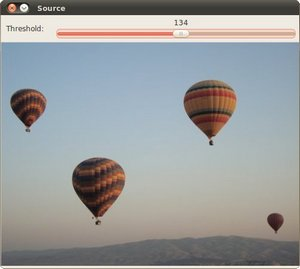
\includegraphics[width=0.8\linewidth]{test}
% %\end{figure}
% \end{frame}

% %------------------------------------------------

% \begin{frame}[fragile] % Need to use the fragile option when verbatim is used in the slide
% \frametitle{Citation}
% An example of the \verb|\cite| command to cite within the presentation:\\~

% This statement requires citation \cite{p1}.
% \end{frame}

% %------------------------------------------------

% \begin{frame}
% \frametitle{References}
% \footnotesize{
% \begin{thebibliography}{99} % Beamer does not support BibTeX so references must be inserted manually as below
% \bibitem[Smith, 2012]{p1} John Smith (2012)
% \newblock Title of the publication
% \newblock \emph{Journal Name} 12(3), 45 -- 678.
% \end{thebibliography}
% }
% \end{frame}

%------------------------------------------------
\section{Closing Remarks}
	\begin{frame}
	\Huge{\centerline{The End}}
	\end{frame}

%----------------------------------------------------------------------------------------

\end{document} 